\subsection{競技の概要}
参加機体は,離着陸エリアから飛行を開始し,ミッションエリアにて以下に述べるミッションを完了したのち,離着陸エリアに帰還する.
最大飛行時間内に複数のミッションを行い,機体の性能および操縦性を評価する項目の総合点を競う.
\subsection{メインミッション}
\paragraph{成功条件}
\begin{itemize}
\item 物資投下エリアに救援物資を1つ投下すること
\item 離着陸エリアに静止すること
  \item ただし,メインミッション終了後でも構わない
\end{itemize}
\paragraph{終了条件}
\begin{itemize}
\item 「投下完了」をコールすること
\item 次のミッションをコールすること
\end{itemize}
\paragraph{得点}
\begin{itemize}
\item メインミッション点 = 時間点 + 投下点 + メインミッション追加点
\item 時間点 = 20×(60-計測時間)
\item 投下点 = エリア1投下点 * 個数 + エリア2投下点 * 個数 + エリア3投下点 * 個数
\item エリア1投下点 = 50
\item エリア2投下点 = 150
\item エリア3投下点 = 300
\item エリア1およびエリア2,エリア3にそれぞれ1つ以上投下したチームにメインミッション追加点 (500点) を与える
\item 投下点は「投下完了」をコールした後に,初めて離着陸エリアに着陸静止したときの救援物資の位置で確定する
\item 計測時間は競技開始からメインミッションの終了条件を満たすまでの時間である
\end{itemize}
\paragraph{付記}
\begin{itemize}
\item エリアの詳細については図\ref{fig::plane::dropArea}を参照すること
\item 投下点はエリア1およびエリア2,エリア3に投下された救援物資のうち合計得点が高くなる最大4つを選択して計算する
\end{itemize}

\subsection{サブミッション}
サブミッションは以下の通り.
\begin{itemize}
\item 8の字飛行
\item 宙返り
\item 無動力滑空
\item 救援物資回収
\item 高所物資回収
\item ポール旋回
\item 帰還
\end{itemize}

ハンズオフ飛行専用ミッションは以下の通り.
\begin{itemize}
\item 水平旋回
\item 上昇旋回
\item 自動物資投下
\end{itemize}

\subsubsection{8の字飛行}
\paragraph{成功条件}
\begin{itemize}
\item 8の字飛行を行うこと(飛行軌跡が「8の字」と認められること)
\item 高度変化が十分小さいこと
\end{itemize}
\paragraph{終了条件}
\begin{itemize}
\item 次のミッションがコールされること
\item 成功条件を満たすこと
\end{itemize}
\paragraph{得点}
\begin{itemize}
\item 8の字飛行点 = 200 + 8の字飛行追加点
\item ハンズオフ飛行で成功条件を満たしたとき,8の字飛行追加点として600点が与えられる
\end{itemize}
\subsubsection{宙返り}
\paragraph{成功条件}
\begin{itemize}
\item 軌道面が地面に対して十分に垂直な宙返りをおこなうこと
\end{itemize}
\paragraph{終了条件}
\begin{itemize}
\item 次のミッションがコールされること
\item 宙返り回数が3回に達すること
\end{itemize}
\paragraph{得点}
\begin{itemize}
\item 宙返り点 = 宙返り回数 * 150
\item 上下方向に機体が1回転して宙返り開始地点に戻ってきたら1回転成功とし,宙返り回数を加算する
\end{itemize}
\paragraph{付記}
\begin{itemize}
\item 連続しての宙返りは認めない
\end{itemize}


\subsubsection{無動力滑空}
\paragraph{成功条件}
\begin{itemize}
\item 7秒以上の滑空飛行を行うこと
\end{itemize}
\paragraph{終了条件}
\begin{itemize}
\item 次のミッションがコールされること
\item 「パワーオン」がコールされること
\item 機体が接地すること
\end{itemize}
\paragraph{得点}
\begin{itemize}
\item 無動力滑空点 = 200 + 50*(滑空時間-10) + 滑空ランキング点
\item 滑空時間は「パワーオフ」のコールから「パワーオン」のコールまでの時間とする
\item 滑空時間の上限は20秒とする
\item 滑空時間の上位には滑空ランキング点を与える
\begin{itemize}
  \item 1位 300点
  \item 2位 200点
  \item 3位 100点
\end{itemize}
\item 同一タイムが複数チーム存在する場合は同順位とし,該当順位の点数をすべての該当チームに与える.
\end{itemize}
\paragraph{付記}
\begin{itemize}
\item 「パワーオン」のコール後に動力飛行をすること
\end{itemize}

\subsubsection{救援物資回収}
\paragraph{成功条件}
\begin{itemize}
\item 他のミッションで物資投下エリアに投下した救援物資のうち1つを,機体に手を
触れない状態で回収し,離着陸エリアに着陸静止すること
  \item 機体が着陸静止した際に救援物資が離着陸エリア内にあれば,着陸の衝撃等で外れても成功とみなす
\end{itemize}
\paragraph{終了条件}
\begin{itemize}
\item 次のミッションがコールされること
  \item ただし,「帰還」を除く
\item 物資投下エリアの救援物資がなくなること
\end{itemize}
\paragraph{得点}
\begin{itemize}
\item 物資回収点 = 回収点+着陸点
\item 回収点と着陸点はともに500点とする
\end{itemize}
\paragraph{付記}
地上走行中に得点エリア外に接地した場合は離着陸エリアからやり直しとする.救援物資を回収した状態であれば,その救援物資は使用不可とする.

\subsubsection{高所物資回収}
\paragraph{成功条件}
\begin{itemize}
\item 指定された場所に設置した救援物資を回収すること
\end{itemize}
\paragraph{終了条件}
\begin{itemize}
\item 次のミッションがコールされること
\end{itemize}
\paragraph{得点}
\begin{itemize}
\item 高所物資回収点=回収点(400点) + 着陸点(600点)
\item 回収点は救援物資を回収したときに与えられる
\item 着陸点は回収した物資を保持したまま離着陸エリアに着陸したときに与えられる
  \item 着陸の衝撃で物資が外れても,物資が離着陸エリア内にあれば得点を認める
\end{itemize}
\paragraph{付記}

\subsubsection{ポール旋回}
\paragraph{成功条件}
\begin{itemize}
\item ポール旋回回数が1以上になること
\end{itemize}
\paragraph{終了条件}
\begin{itemize}
\item 次のミッションがコールされること
\end{itemize}
\paragraph{得点}
\begin{itemize}
\item ポール旋回点 = ポール旋回回数 * 150 + 連続旋回回数 * 100
\end{itemize}
\paragraph{付記}
\begin{itemize}
\item ラインA→ラインB→ラインAの順で通過することでポール旋回回数が加算される
\item ポール旋回回数は3回を上限とする
\item 旋回は途中から開始しても構わない
\item ラインAは離着陸エリアとミッションエリアの境界線とする
\item ラインBは体育館壁面の垂線でポールと壁面を結ぶ線とする
  \item 図\ref{fig::plane::poleTurn}を参照すること
\item 機体が離着陸エリアで静止しているときにポールの取り外し,取り付けをピットメンバーがしてもよい
\end{itemize}

\subsubsection{水平旋回}
\paragraph{成功条件}
\begin{itemize}
\item ハンズオフ飛行による水平旋回を行うこと
\item 水平旋回中の高度変化が十分小さいこと
\end{itemize}
\paragraph{終了条件}
\begin{itemize}
\item 次のミッションがコールされること
\item 水平旋回回数が2回に達すること
\end{itemize}
\paragraph{得点}
\begin{itemize}
\item 水平旋回点 = 水平旋回回数 * 200 + 水平旋回追加点(200点)
\item 水平旋回追加点は連続して2回旋回した場合に加算される
\end{itemize}

\subsubsection{上昇旋回}
\paragraph{成功条件}
\begin{itemize}
\item ハンズオフ飛行による上昇旋回を行うこと
\end{itemize}
\paragraph{終了条件}
\begin{itemize}
\item 次のミッションがコールされること
\item 成功条件を満たすこと
\end{itemize}
\paragraph{得点}
\begin{itemize}
\item 上昇旋回点 = 1000
\end{itemize}
\paragraph{ミッションプロセス}
\begin{enumerate}
  \item 「上昇旋回開始」のコールとともに,ハンズオフ飛行に切り替える
  \item 競技エリアにおけるポール以下の高度を保ったまま水平旋回を2周行う
  \item 旋回しながら高度を上げ,キャットウォーク以上の高度に到達する
  \item キャットウォーク以上の高度を保ったまま,水平旋回を2周行う
\end{enumerate}
\paragraph{付記}
\begin{itemize}
  \item 旋回方向はミッション記入用紙に記入した方向のみ認められる
  \item 旋回方向はサブミッション「水平旋回」と逆方向のみ認められる
  \item 機体の一部でも指定された高度領域を違反したと判断された場合,上昇旋回と認めない
\end{itemize}

\subsubsection{自動物資投下}
\paragraph{成功条件}
\begin{itemize}
  \item ハンズオフ飛行で離着陸エリアから離陸した機体が物資投下エリアに救援物資を投下すること
  \item 操縦者による手動操縦で離着陸エリア内で接地し機体が完全に静止すること
\end{itemize}
\paragraph{終了条件}
\begin{itemize}
  \item ミッション中止のコールがなされること
  \item 救援物資を投下する前に,手動操縦に切り替えること
  \item 離着陸エリア外で接地すること
  \item 離着陸エリアに着陸・静止すること
\end{itemize}
\paragraph{得点}
\begin{itemize}
  \item 自動物資投下点 = 自動離陸点 + 自動物資投下点 + 着陸点
  \item 離着陸エリア内で離陸に成功したとき自動離陸点として200点を与える
  \item ハンズオフ飛行中に救援物資を物資投下エリアに投下できた場合,自動投下点として1000点を与える
  \item 離着陸エリア内で接地し機体が完全に静止したとき着陸点として100点を与える
\end{itemize}
\paragraph{付記}
\begin{itemize}
  \item ミッション開始から1分以内に離陸させること
  \item 本ミッションに挑戦する時間は飛行時間として計測されない
  \item レフェリーの指示後,「自動離着陸開始」のコールとともに,ハンズオフ飛行に切り替える
  \item ハンズオフ飛行に切り替えた後,送信機から手を離す
  \item 物資投下後に手動操縦に切り替え着陸すること
  \item このミッション挑戦中は機体回収できない
\end{itemize}

\subsubsection{帰還}
\paragraph{成功条件}
\begin{itemize}
\item ミッションエリアから離着陸エリア内で接地して機体が完全に静止すること
\end{itemize}
\paragraph{終了条件}
\begin{itemize}
\item 機体が静止すること
\end{itemize}
\paragraph{得点}
\begin{itemize}
\item 帰還点 = 着陸点(50点)+停止点(100点)+滑走路内着陸点(100点)
\item 離着陸エリア内に接地した場合,着陸点として50点を加算する
\item 離着陸エリア内で静止した場合,停止点として100点を加算する
\item 滑走路内で着陸静止した場合,滑走路内着陸点として100点を加算する
\item 接地物に接触した場合,以降の得点を認めない
\end{itemize}
\paragraph{付記}
\begin{itemize}
\item 帰還が終了したとき競技を終了とする
\item ただし,「自動物資投下」がコールされたとき同ミッションへの挑戦を認める
\end{itemize}

\subsection{フィールド}
\subsubsection{物資投下エリア}
物資投下エリア \ref{fig::plane::dropArea} に示す.
黄色の枠の内側が物資投下エリアである.
赤の円の内側を除く,緑色の枠の内側を投下エリア1とする.
赤の円の内側を投下エリア2とする.
青の枠の内側を投下エリア3とする.
当日のフィールドでは図と同じ位置にマーカーを置く.

\begin{figure}[bh]
  \centering\includegraphics[width = 50mm,angle=90]{./plane_dropArea.png}
  \caption{物資投下エリア}
  \label{fig::plane::dropArea}
\end{figure}

\subsubsection{ポール旋回}
図 \ref{fig::plane::poleTurn} にポール旋回に用いるラインBを青線で示す.
\begin{figure}[h]
  \centering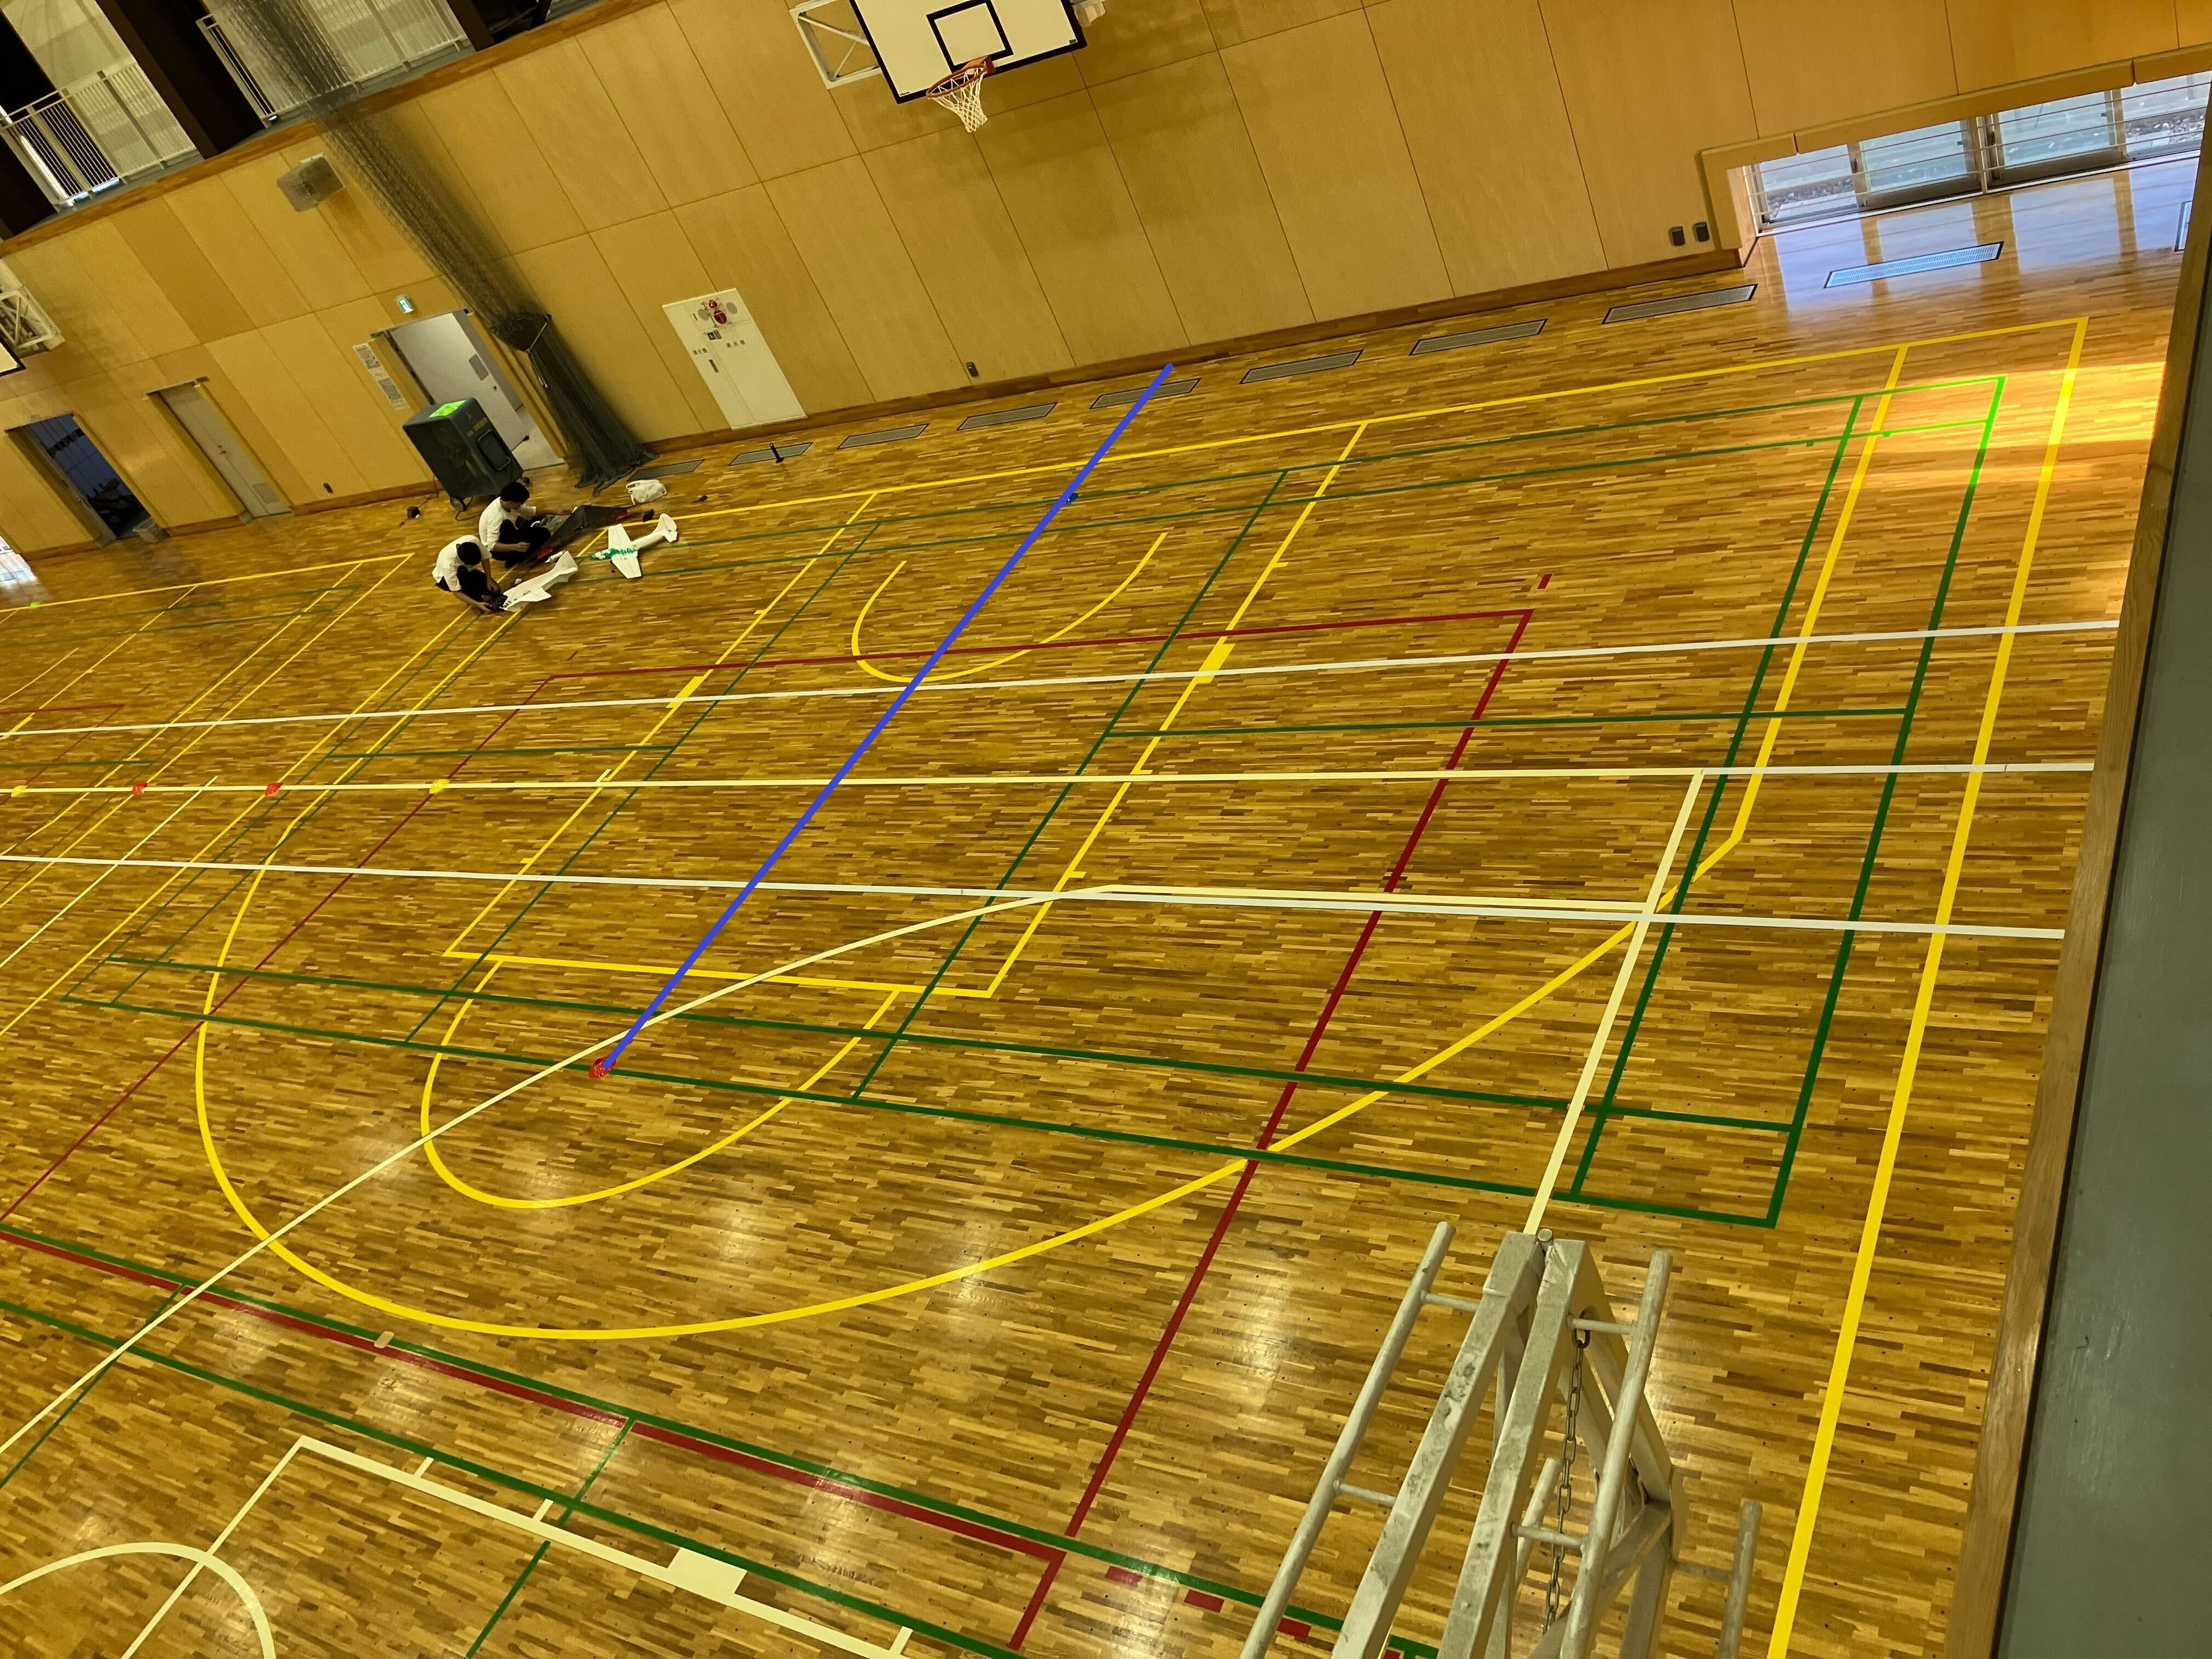
\includegraphics[width=70mm]{plane_poleTurn.jpg}
  \caption{ポール旋回}
  \label{fig::plane::poleTurn}
\end{figure}

\subsubsection{離着陸エリア}
図 \ref{fig::plane::landingZone} に離着陸エリアを示す.
\begin{itemize}
  \item オレンジの斜線部を滑走路とする
  \item 緑の斜線部と滑走路を合わせて離着陸エリアとする
  \item 体育館の壁面は離着陸エリア外とする
\end{itemize}
\begin{figure}[htb]
  \centering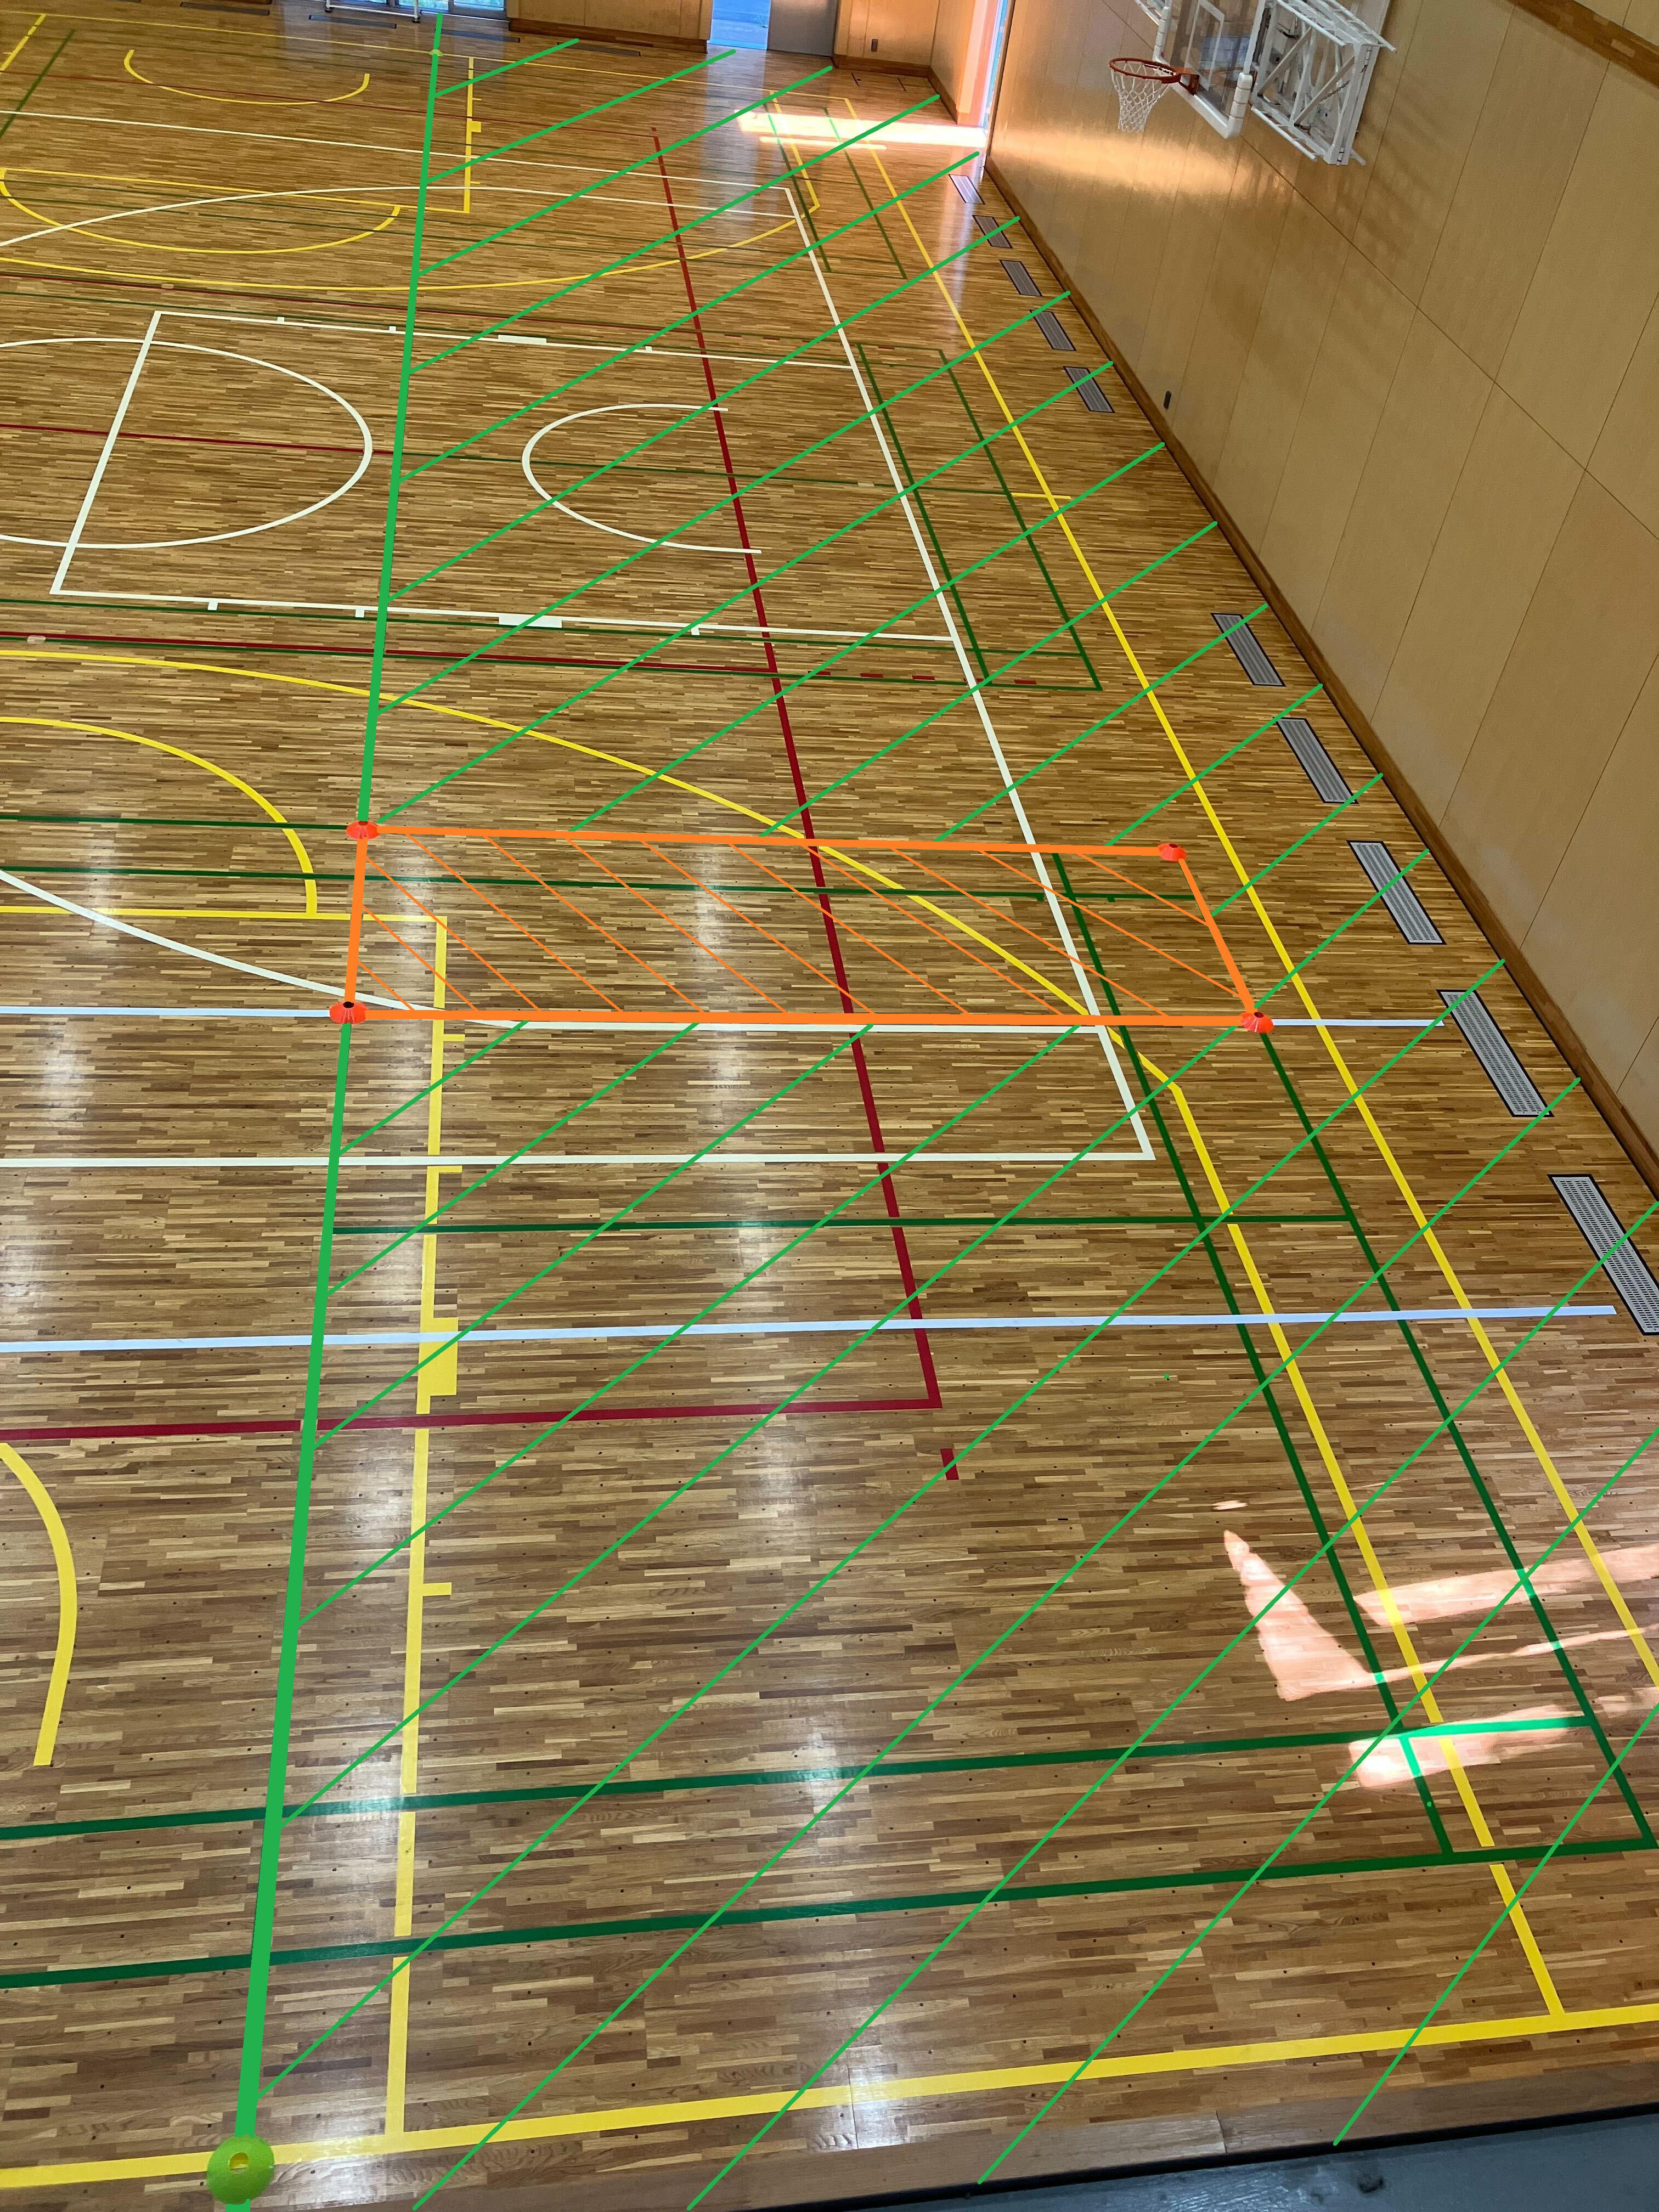
\includegraphics[width = 50mm,angle=90]{./plane_landingZone.jpg}
  \caption{離着陸エリア}
  \label{fig::plane::landingZone}
\end{figure}
\newpage